\section{Introduction}\label{sec:intro}


Let $X$ be a smooth complex projective variety. The Hodge conjecture asserts
that the cycle class map
\[
  \cl^{p}_{X}\colon \CH^{p}(X)_{\QQ}\longrightarrow \Hdg^{p}(X)
  \coloneqq H^{2p}(X,\QQ)\cap H^{p,p}(X)
\]
is surjective for every $p$. For $p=1$ this is the theorem of Lefschetz on
$(1,1)$ classes.%
\footnote{The rational coefficients are essential. The theorem of Lefschetz
holds integrally in degree two, but the integral analogue fails in higher
degree: Atiyah and Hirzebruch found torsion classes of type $(p,p)$ that are
not classes of cycles, and Koll\'ar found non-torsion ones. Every statement in
this paper concerns $\QQ$-coefficients.}
Beyond degree two the best understood Hodge classes are those of abelian
varieties, and the first of them that divisors do not produce are the Weil
classes. Weil exhibited them on abelian varieties with an action of an
imaginary quadratic field whose two eigenspaces on the tangent space have the
same dimension, showed that they are Hodge classes outside the subring
generated by divisor classes, and proposed them as test cases for the Hodge
conjecture \cite{Weil77}. The construction works for every CM field $F$ in
place of the quadratic one. On a general abelian variety of Weil type the
Hodge ring is generated by divisor classes together with the Weil classes, a
flat $F$-line of classes of middle degree, so for these varieties the Hodge
conjecture is the algebraicity of the Weil classes.

Markman proved that the Weil classes are algebraic on the abelian sixfolds of
split Weil type for every imaginary quadratic field, and, through a product
argument of Schoen \cite[Proposition~10]{Sch98}, on every abelian fourfold of
Weil type \cite{Mar25a,Mar25b}.%
\footnote{In the normalisation of \Cref{def:disc} the discriminant is the
class of $(-1)^{n}\det H$ in $\QQ^{\times}_{>0}/\Nm_{K/\QQ}(K^{\times})$.
Markman uses the class of $\det H$ itself, in which the same sixfolds have
discriminant $(-1)^{3}=-1$.}
With the description of the Hodge rings of abelian varieties of dimension at
most five by Moonen and Zarhin \cite{MZ99}, this gives the Hodge conjecture
for abelian fourfolds and fivefolds. His sheaves are built from secant sheaves
on an abelian variety of half the dimension, and they extend along the family
because they satisfy an equivariant form of semiregularity. This paper is
about the set of members of a family on which a flat Hodge class is
algebraic, which we call its algebraic locus. For the Weil classes we
determine it for every CM field and every dimension at once. The companion
paper \cite{paperII} determines what closing that locus requires of a single
object at a single point and examines the objects that the known
constructions supply, and the companion paper \cite{paperIII} places the
Weil classes inside the whole conjecture.

\subsection{The main theorem}

Fix a CM field $F$ of degree $2m$, an integer $n\ge2$ and a discriminant
$\delta$. The abelian varieties of $(F,n,\delta)$-Weil type are the members of
one family over a connected period domain $\cD_{F}$ of dimension $mn^{2}$, a
product of $m$ copies of the bounded symmetric domain of $\SU(n,n)$, and their
Weil classes form a flat local system of rank $2m$ over it
(\Cref{setup:cmfield}, \Cref{prop:cmweil}). We call the set
\[
  \Sigma_{F}=\{\,s\in\cD_{F}:\text{the Weil classes of }A_{s}\text{ are
  algebraic}\,\}
\]
the \emph{algebraic locus} of the family. A property holds for the
\emph{very general member} if it holds outside a countable union of proper
closed analytic subsets of $\cD_{F}$.%
\footnote{A subset of $\cD_{F}$ is \emph{meagre} if it is contained in a
countable union of closed subsets with empty interior. Since $\cD_{F}$ is a
complex manifold, the Baire category theorem shows that a meagre set has
dense complement, so a statement that holds off a meagre set holds on a dense
set of members; the very general members are those off a particular meagre
set, a countable union of proper analytic subsets.}

\begin{theorem}[Main theorem]\label{thm:main}
For every CM field $F$, every $n\ge2$ and every discriminant $\delta$, the
algebraic locus $\Sigma_{F}$ of the Weil classes has the following
properties.
\begin{enumerate}[label=\textup{(\roman*)},leftmargin=2.6em,itemsep=2pt]
\item It contains an explicit point $s_{0}$ at which $A_{s_{0}}$ is isogenous
  to a product of abelian varieties with complex multiplication by $F$, and
  at which the Weil classes are polynomials with rational coefficients in
  divisor classes.
\item It is dense in $\cD_{F}$.%
\footnote{Density comes from the Hecke orbit of $s_{0}$: the group
$G_{F}(\QQ)$ of rational points of the unitary group of the hermitian form
acts on $\cD_{F}$ through isogenies that respect the $F$-action and the
polarisation up to a scalar, so it preserves the algebraicity of the Weil
classes, and the closure of $G_{F}(\QQ)$ contains the identity component of
$G_{F}(\RR)$, which acts transitively on $\cD_{F}$; the proof uses the
rational isotropic vectors of the hermitian form, which exist by the Hasse
principle.}
\item It is the preimage of a countable union of Zariski closed subsets of the
  Shimura variety of the family, and either $\Sigma_{F}=\cD_{F}$ or
  $\Sigma_{F}$ is meagre.
\item The following are equivalent: $\Sigma_{F}$ is closed; $\Sigma_{F}$ has
  an interior point; the Weil classes are algebraic on every member of the
  family; the Hodge conjecture holds for the very general member of the
  family.
\end{enumerate}
\end{theorem}

For $n=1$ the Weil classes have degree two and are algebraic by the theorem
of Lefschetz, and all four statements hold trivially. The proof of
\Cref{thm:main} is completed in \Cref{sec:cmfields}, after the imaginary
quadratic case has been treated in full in \Cref{sec:construction,sec:basepoints,sec:propagation}.
\Cref{fig:mainlocus} draws the picture it describes: a connected domain, a
dense set built from one explicit point, and a decomposition of that set into
countably many closed algebraic strata.


The theorem carries the Hodge conjecture for the very general abelian variety
of Weil type, for every CM field, every dimension and every discriminant, to
a single topological statement about one explicit set: the dense set
$\Sigma_{F}$, which is a countable union of closed algebraic subsets of a
connected Shimura variety, has to be closed. The paper is organised around
that statement. \Cref{sec:conventions,sec:weiltype,sec:explicit} fix the
conventions, the families and the explicit form of the Weil classes;
\Cref{sec:characters,sec:fm,sec:divisor,sec:numerology,sec:semireg,sec:hyperplane,sec:ks,sec:reduction,sec:escape}
show why the classical constructions do not produce Weil classes and what any
construction must look like; \Cref{sec:construction,sec:basepoints,sec:propagation}
prove the theorem for imaginary quadratic fields, where everything can be
written in coordinates; and \Cref{sec:cmfields} completes the proof for every
CM field. The companion papers take the statement further: \cite{paperII}
shows that one semiregular object at one base point would close
$\Sigma_{F}$, computes the semiregularity condition exactly and excludes the
objects of the classical constructions, and \cite{paperIII} shows that the
whole Hodge conjecture is two statements about such loci.

\begin{figure}[htbp]
\centering
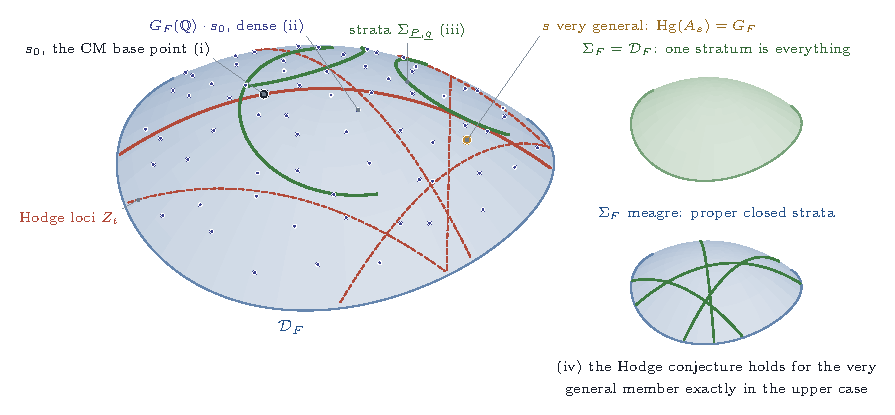
\includegraphics[width=\textwidth]{fig_mainlocus}
\caption{The algebraic locus of \Cref{thm:main}, drawn over a real slice of the
period domain $\cD_{F}$. Left: the explicit CM base point $s_{0}$ of part (i);
its Hecke orbit $G_{F}(\QQ)\cdot s_{0}$, which is dense by part (ii); three of
the strata $\Sigma_{\underline{P},\underline{q}}$ of part (iii), each closed
and algebraic, through points of the orbit; the Hodge loci $Z_{t}$, dashed,
one of them through $s_{0}$, off which the Hodge group of the member is all of
$G_{F}$ (\Cref{lem:cmgeneric}); and a very general point $s$. Right: the two
cases of the dichotomy of part (iii). By part (iv) the Hodge conjecture holds
for the very general member exactly in the upper case, where one stratum is
the whole domain.}
\label{fig:mainlocus}
\end{figure}


\subsection{The proof}

The first step is a base point. In \Cref{thm:cmbasepoint} the member $A_{s_{0}}$
is isogenous to $B_{\Phi}^{\,n}\times B_{\bbar\Phi}^{\,n}$, where $B_{\Phi}$ is
an abelian $m$-fold with complex multiplication by $F$ of a CM type determined
by the polarisation, and the Weil classes there are written out as
polynomials with rational coefficients in $F$-balanced divisor classes. For
an imaginary quadratic field $K$ there is a second base point in every family,
with quaternionic multiplication: whenever an algebra $(-d,b)_{\QQ}$ with
$b>0$ acts compatibly with $K$, the Weil line is spanned by the real and
imaginary parts of $\Theta^{n}$ for an explicit $(1,1)$ class $\Theta$, and
the discriminant of the family is the class of $b^{n}$, which can be any
discriminant (\Cref{thm:divcriterion}, \Cref{thm:quatweil},
\Cref{thm:everyfamily}). Products of abelian surfaces of Weil type give a
third, since the Weil class is multiplicative:
$\omega(A_{1})\,\omega(A_{2})=\omega(A_{1}\times A_{2})$ for the
$K$-valued Weil class $\omega$ (\Cref{thm:weilmult}, \Cref{thm:everyn}). None
of these base points uses anything beyond the theorem of Lefschetz on $(1,1)$
classes.

The second step moves the base point. An element of $G_{F}(\QQ)$, where
$G_{F}=\Res_{F_{0}/\QQ}\SU(V,H)$ and $F_{0}$ is the totally real subfield,
induces after clearing denominators an isogeny between two members and fixes
the Weil classes, so $\Sigma_{F}$ is a union of $G_{F}(\QQ)$-orbits
(\Cref{lem:Ginvariance}). The hermitian form is isotropic by the Hasse
principle, the rational points of the unipotent radicals of the parabolic
subgroups are dense in their real points, and these real points generate the
identity component of $G_{F}(\RR)$; so every orbit is dense
(\Cref{prop:densealg}, \Cref{thm:cmpropagation}(ii)).

The third step is properness. The relative Hilbert scheme of the universal
family, for one tuple of Hilbert polynomials, is proper over the Shimura
variety,%
\footnote{By Grothendieck's construction the Hilbert scheme of a projective
morphism, for a fixed Hilbert polynomial, is projective over the base; here
the base is the Shimura variety of the family, after a level structure that
makes the universal family exist, and the morphism is the universal abelian
scheme.}
and the class of a flat family of cycles is locally constant, so the
set of points at which a Weil class is represented by cycles with prescribed
Hilbert data is Zariski closed; $\Sigma_{F}$ is the countable union of these
strata (\Cref{thm:closedlocus}). The Baire category theorem then gives the
dichotomy of part (iii) (\Cref{cor:allornothing}). Part (iv) needs one more
fact, that the very general member has Hodge group $G_{F}$; we prove it
directly, from the simplicity of the real factors $\SU(n,n)$
(\Cref{lem:cmgeneric}, \Cref{cor:verygeneral}).

For an imaginary quadratic field everything can be written in coordinates.
On the standard model of \Cref{sec:explicit}, built from a $K$-vector space of
dimension $2n$ with a hermitian form of signature $(n,n)$, the Weil line has
the integral basis
\[
  \omega_{1}=\sum_{|T|\ \mathrm{even}}(-1)^{|T|/2}d^{\,n-|T|/2}\,w^{(T)},
  \qquad
  \omega_{2}=\sum_{|T|\ \mathrm{odd}}(-1)^{(|T|-1)/2}d^{\,n-(|T|+1)/2}\,w^{(T)},
\]
where $T$ runs over the subsets of $\{1,\dots,2n\}$ and $w^{(T)}$ is the
monomial taking $y_{j}$ for $j\in T$ and $x_{j}$ otherwise
(\Cref{thm:explicitgens}). A member with Hodge group $\SU(V,H)$ has exactly
three Hodge classes in degree $2n$ and one in every other degree
(\Cref{thm:hdgcount}), so the Hodge conjecture for it, in every degree at
once, is the algebraicity of the one class $\omega_{1}$, with $2^{2n-1}$
integer coefficients (\Cref{cor:whatisleft}). By Deligne's theorem
\cite{Del82} that class is absolutely Hodge at every point,%
\footnote{A class is absolutely Hodge if its image under every automorphism
$\sigma$ of $\CC$, through the comparison of Betti cohomology with
algebraic de Rham cohomology of the conjugate variety $X^{\sigma}$, is again
a Hodge class. Algebraic classes have this property, so it is a necessary
condition for algebraicity; Deligne proved it for every Hodge class on an
abelian variety.}
and the Hodge
conjecture for the family is equivalent to its algebraicity at every point of
one connected domain (\Cref{cor:exactform}).


\subsection{The classical constructions}

\Cref{sec:characters,sec:fm,sec:divisor,sec:numerology,sec:semireg,sec:hyperplane,sec:ks,sec:reduction,sec:escape} explain why two classical lines of attack do not
produce Weil classes, and the explanations are different in kind. The first
imports an object from a projective space, restricts it to the dual abelian
variety and transports it back by the Fourier--Mukai transform. Its Chern
character stays in the subring generated by the polarisation
(\Cref{thm:divisor}), because the cohomological transform carries powers of
the dual polarisation to rational multiples of powers of the polarisation in
closed form (\Cref{thm:fmtheta}); and a construction equivariant for the
field lands in the isotypic component of the norm character, which the Weil
line misses, since it sits at the two ends of the grading
(\Cref{thm:character}). The second is induction on dimension through
hyperplane sections, and the restriction map kills every primitive class of
middle degree (\Cref{thm:hyperplane}); below the middle degree the return
trip is the Lefschetz standard conjecture (\Cref{thm:returntrip}). The
Kuga--Satake construction, which changes the variety rather than cutting it,
reaches the Weil line only in dimension two (\Cref{prop:normpart}).%
\footnote{The construction attaches to a polarised Hodge structure $T$ of
weight two with $h^{2,0}=1$ an abelian variety $A$ with
$H^{1}(A,\QQ)=C^{+}(T)$, the even Clifford algebra, and an embedding of
$T$ into $\End(H^{1}(A,\QQ))$ by Hodge structures, which is a Hodge class on
the product of a variety carrying $T$ with $A\times A$; the Kuga--Satake
Hodge conjecture asks that this class be algebraic.} A rational
class of the Weil line has a $\Kx$-orbit spanning a plane, so any
construction reaching it must be bilinear in a pair of inputs exchanged by
$\Gal(K/\QQ)$ (\Cref{prop:orbitplane}), and Markman's construction is of that
kind.


\subsection{The companion papers}

By \Cref{thm:main}(iv) the Hodge conjecture for the very general member of a
Weil family is the closedness of $\Sigma_{F}$, and by (iii) it is enough to
show that one stratum has an interior point. Two statements would do this.
The first bounds the Hilbert data of the cycles along the orbit of the base
point (\Cref{thm:degreebound}); it is equivalent to its conclusion
(\Cref{thm:p1equivalent}), and it is needed only along one sequence of CM
points that leaves every proper special subvariety, which exists in the
orbit (\Cref{thm:escape}). The second is semiregularity: a perfect complex
at one base point whose Chern character is a nonzero multiple of a Weil
class plus a polynomial in the polarisation, and whose semiregularity map is
injective, extends along the whole family. The companion paper
\cite{paperII} proves this (\cite[Theorem~2.3]{paperII}), computes the
injectivity condition as one number, shows that it is never met when the
Chern character is exactly a Weil class, for any CM field, computes it
exactly for quartic CM fields, examines the secant objects of the split
member, the convolutions of line bundles and the supports of a complex
meeting the criterion. The companion paper \cite{paperIII} shows that the
Hodge conjecture is equivalent to two statements about algebraic loci, one on
abelian varieties and one on the classes reached from them by
correspondences, proves each where it can be proved, and proves the
conjecture itself for the very general complete intersection of diagonal
quadrics of Vandermonde type. The annihilator computation of
\Cref{sec:semireg}, which shows that no object on which $H^{2}(\cO_{A})$ acts
faithfully is semiregular, is the first step of that analysis and is proved
here because it uses only the explicit form of the classes.

Every proof is written to be checked by hand. Where an argument rests on a
finite calculation, the calculation is given where it is used, as an explicit
identity, a determinant or a case analysis. The archive \cite{BMB26} holds
programs that repeat much of this arithmetic and a Lean~4 certificate of
part of it; no statement of the paper rests on them.
